\begingroup
\clearpage\thispagestyle{empty}
\noindent
\begin{tikzpicture}
\draw[line width=.65pt] (0,0) rectangle (\textwidth,224mm);
\draw[line width=.3pt] (6mm,6mm) rectangle (\textwidth-6mm,218mm);
\node[anchor=north,inner sep=0pt,text width=\dimexpr\textwidth-16mm\relax,align=center] at (.5\textwidth,197mm) {%
{\Large\bfseries CARL FRIEDRICH GAUSS}\par\vspace{12mm}
{\Huge\bfseries WERKE}\par\vspace{16mm}
{\large\textls[200]{NEUNTER BAND}}\par\vspace{17mm}
{\footnotesize HERAUSGEGEBEN}\par\vspace{8mm}
{\scriptsize VON DER}\par\vspace{9mm}
{\normalsize\bfseries KÖNIGLICHEN GESELLSCHAFT DER WISSENSCHAFTEN}\par\vspace{7mm}
{\scriptsize ZU}\par\vspace{6mm}
{\large\textls[180]{GÖTTINGEN}}\par\vspace{28mm}
{\small IN COMMISSION BEI B. G. TEUBNER IN LEIPZIG}\par\vspace{3mm}
{\small 1903.}};
\end{tikzpicture}\par
\clearpage\null
\clearpage\thispagestyle{empty}
\vspace*{76mm}
\begin{center}
{\Large CARL FRIEDRICH GAUSS WERKE}\par\vspace{12mm}
{\large BAND IX.}
\end{center}
\clearpage\null
\clearpage\thispagestyle{empty}
\begin{center}
\vspace*{10mm}
{\Large CARL FRIEDRICH GAUSS}\par\vspace{10mm}
{\Huge\bfseries WERKE}\par\vspace{14mm}
{\large\textls[200]{NEUNTER BAND.}}\par\vspace{11mm}
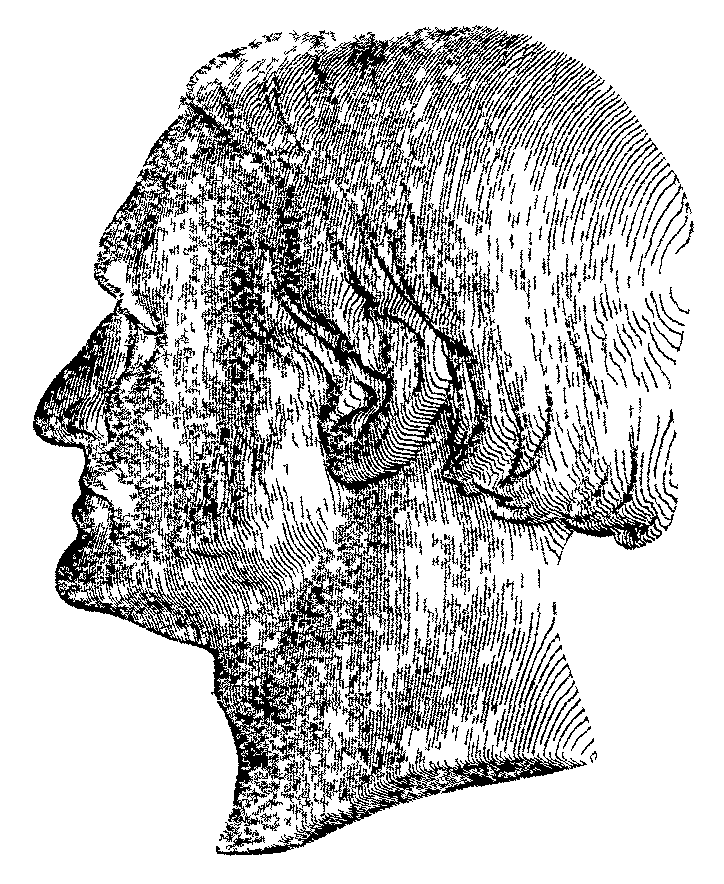
\includegraphics[width=44mm]{gauss_historical_portrait.png}\par\vspace{18mm}
{\footnotesize HERAUSGEGEBEN}\par\vspace{3mm}
{\scriptsize VON DER}\par\vspace{3mm}
{\small KÖNIGLICHEN GESELLSCHAFT DER WISSENSCHAFTEN}\par\vspace{3mm}
{\scriptsize ZU}\par\vspace{4mm}
{\large\textls[180]{GÖTTINGEN.}}\par\vspace{3mm}
{\small IN COMMISSION BEI B. G. TEUBNER IN LEIPZIG.}\par\vspace{3mm}
{\small 1903.}
\end{center}
\clearpage\null
\endgroup
